
\subsection{El fichero \texttt{/tmp/conf.tmp}} \label{append:F_conf.tmp}

El fichero \verb|conf.tmp| es un fichero temporal en el que se escriben las nuevas configuraciones a la espera de ser aplicadas por el configurador. El ciclo de vida de este fichero se describe en el diagrama de secuencia de la figura \ref{fig:lms11-conf.tmp}. En resumen, el instalador configura el equipo mediante una aplicación, la cual se encarga de escribir el fichero en disco con un formato predeterminado para luego notificar al \textit{configurador}, quien lee y aplica la nueva configuración. La aplicación puede ser web, como en el caso del LM7, o de escritorio, como en el caso de nuestro sistema (LM11). En este último caso, la aplicación no escribe los datos directamente en disco ya que es un sistema externo al limitador, en su lugar, se pasa por la API del limitador, enviándole los datos de la nueva configuración. La API comprueba y escribe los datos en disco, para finalmente dar paso al \textit{configurador}.

!!! TODO
%\begin{figure}[h]
%	\centering
%    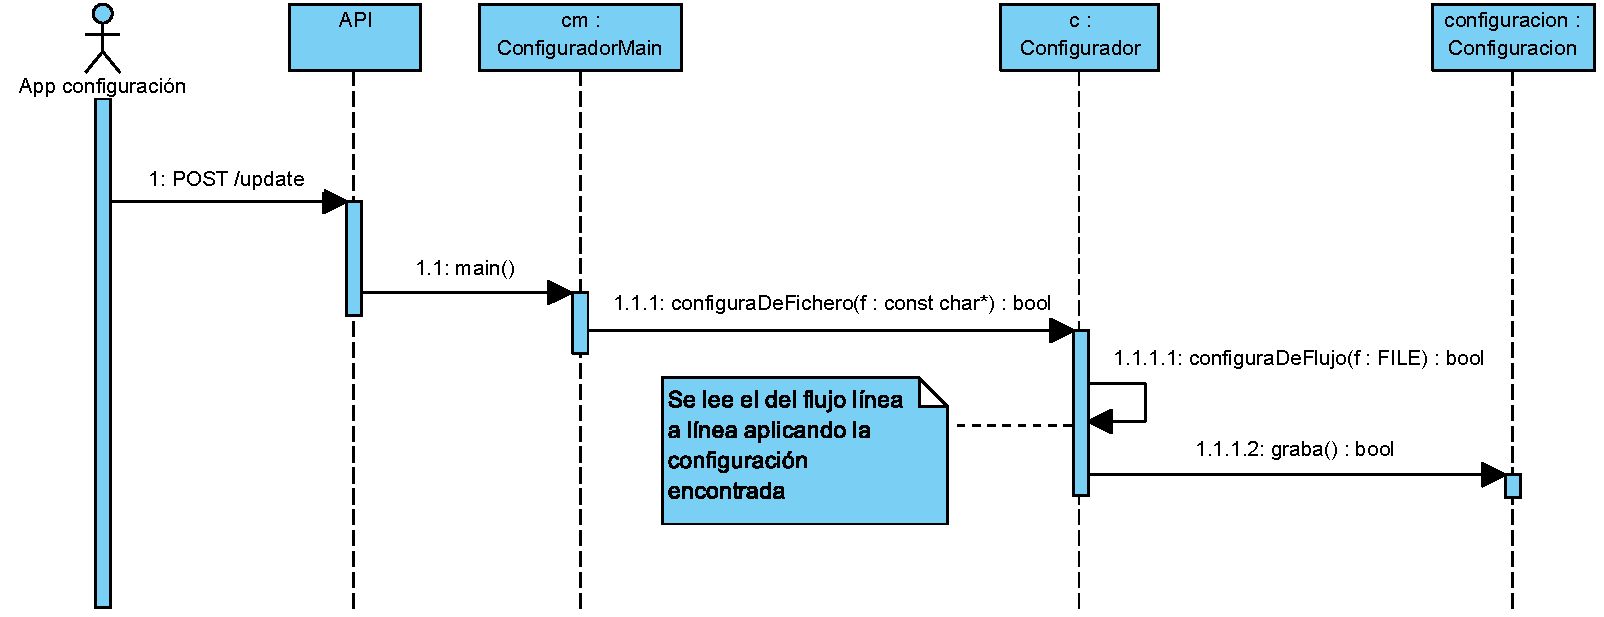
\includegraphics[width=0.55\textwidth]{figuras/lms11-conf.tmp}
%    \caption{Diagrama de secuencia para actualizar la configuración en el LM11.}
%    \label{fig:lms11-conf.tmp}
%\end{figure}

En el listado inferior se muestra cada una de las propiedades configurables del limitador y su formato en el fichero  \verb|conf.tmp|. Cada una de las propiedades debe ocupar una y solo una línea en el fichero, y no es obligatorio configurarlas todas, ya que el configurador solo actualiza las propiedades que encuentra en el fichero.

Nota: las falta de tildes en los nombres de las propiedades es intencionada.
\begin{itemize}
	\item Identificacion \$char[50]
	\item Version \$char[50]
	\item Activacion \$bool
	\item Desactivacion \$bool
	\item Local \$char[50]
	\item Direccion \$char[255]
	\item Telefono \$char[50]
	\item Persona \$char[50]
	\item Ayuntamiento \$char[50]
	\item Distribuidor \$char[50]
	\item BloqueoDeAudio \$bool
	\item Predictivo \$bool
	\item Laeq \$int
	\item Tiempo \$int
	\item Atenuación \$float
	\item Pasos \$int
	\item AtPorBanda \$float
	\item Password \$char[50]
	\item Control \$int \footnote{0: mic, 1: línea, 2: mixto}
	\item RangoDePenalización \$float
	\item PartesDeCompresor \$int
	\item atenuacionMinima  \$float
	\item coeficienteDeThreshold \$float
	\item Norma \$hI \$hF \$mD \$mN \$mRD \$mRN \footnote{horaIni, horaFin, maxDiurno, maxNocturno, maxRecepcionDiruno, maxRecepcionNocturno}
	\item Aislamiento \$float[n] \footnote{n = nº de bandas de frecuencia. LM7: 8, LM9 y LM11: 31} \footlabel{arraySeparadoPorComas}{Array separado or comas, sin espacios.}
	\item Margenes \$float[n] \footnote{Solo en LM9.} \footref{arraySeparadoPorComas}
	\item UsarControlDeRecepcion \$bool
	\item PinkNoiseLevel \$float
	\item SessionStartThreshold \$float
	\item SessionEndThreshold \$float
	\item UsarControlFrecuancial \$bool
	\item ControlarCadaFrecuencia \$bool
	\item UsarNormativaExtendidad \$bool
	\item LimiteSemanalDiurno \$float[7] \footref{arraySeparadoPorComas}
	\item LimiteSemanalNocturno \$float[7] \footref{arraySeparadoPorComas}
	\item LimiteSemanalRecepcionDiurno \$float[7] \footref{arraySeparadoPorComas}
	\item LimiteSemanalRecepcionNocturno \$float[7] \footref{arraySeparadoPorComas}
	\item FestivosClear
	\item Festivo \$tipo(int)\footnote{0: desactivado, 1: activado, 2: primer lunes del mes} \$día(int) \$numDía(int) \$mes(int) \$horaIni(int) \$horaFin(int) \$minIni(int) \$minDuración(int) \$maxEmisión(float) \$maxRecepción(float)
	\item equipoInstalado \$char[9999]
	\item otrosValores \$char[4096]
\end{itemize}

Durante la implementación del LM11 se modificaron algunos de los nombres por otros más significativos:
\begin{itemize}
	\item Laeq $\rightarrow$ MedidasPorCiclo
	\item Atenuacion $\rightarrow$ AtenuacionMaxima
	\item Tiempo $\rightarrow$ TiempoBajoMaximo
	\item atenuacionMinima $\rightarrow$ AtenuacionMinima
\end{itemize}

También se añadieron propiedades nuevas que eran necesarias poder configurar:
\begin{multicols}{2}
\begin{itemize}
	\item SessionStartDelay \$int
	\item SessionEndDelay \$int
	\item Licencia \$char[150]
	\item Expiración \$time\_t
	\item Sala \$char[150]
	\item Fuentes \$char[150]
	\item Altavoces \$char[150]
	\item Etapas \$char[150]
	\item Crossovers \$char[150]
	\item Ecualizadores \$char[150]
	\item Mesas \$char[150]
\end{itemize}
\end{multicols}

Los siguientes datos estaban disponibles para su configuración en las versiones LM7 y LM9, pero se eliminaron en la LM11.
\begin{itemize}
	\item Boanerges.Server
	\item Boanerges.Port
	\item Boanerges.IncomingMessagesEncryptionKey
	\item Boanerges.OutcomingMessagesEncryptionKey
	\item Boanerges.Secret
	\item Boanerges.ServerRevision
	\item equipoInstalado
	\item otrosValores
\end{itemize}
